\section{Introduction}

Traditional control model
Anthony’s pyramid
• Strategic control à overall business
objectives
• Management control à financial
resource management (budgeting vs.
strategic objectives)
• Operational control à operating
activities (vs. business objectives and
financial resources)
\begin{figure}[H]
    \centering
    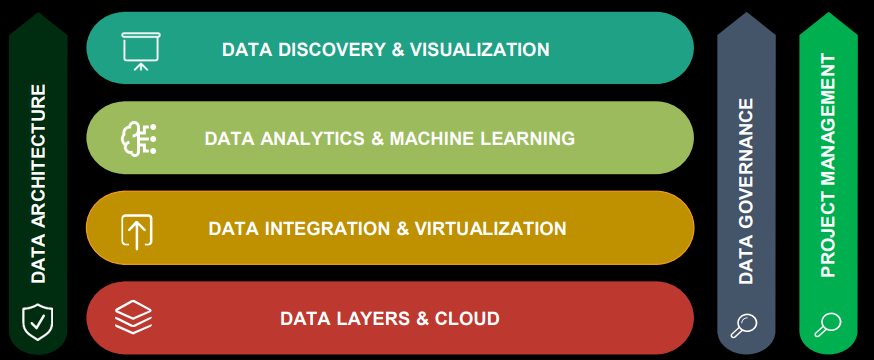
\includegraphics[width=0.5\linewidth]{images/bis3.png}
    \caption{Anthony’s pyramid}
\end{figure}
Functional map of executive information systems
Financial
performance
Planning
Budgeting
Reporting
Activity based
costing
Process
performance
Management
dashboards
Input-output
process models
Clients and
markets
Executive CRM
Analytical CRM
Innovation
and critical
resources
Strategic
planning
Strategic
control
(balanced
scorecard)
Information
to
stakeholders
Communication
Portals
Control models and variables
2009
Financial
performance
Costs
Revenues
Value added
Management
accounting
Value-based
management
Process
performance
Process
efficiency
Process
effectiveness
KPI models
(key
performance
indicators)
Clients and
markets
Loyalty
Profitability
Market
analysis
Client
clustering
Innovation
and critical
resources
Strategic
initiatives
Strategic
resources
Strategic
business
management
framework

\subsubsection{Innovation and critical resources}
Strategic planning • Definition of strategic position tables (e.g. feature-benefit
table of new products)
• Definition of model for value-based management
• Simulation tools for strategic scenarios
• Definition of budget, schedule and deliverables of strategic
initiatives
• Definition of links with other systems (e.g. Balanced Score
Card, Planning, Budgeting, Reporting)
Strategic control
(balanced
scorecard)
• Monitoring of actions and strategic indicators (balanced
scorecard)
• Monitoring of relationships among different indicators in the
balanced scorecard (simulation)
• Report analysis
• Report summary and sharing
• Continuous negotiation of management objectives
• Incentive distribution (consistent with strategic objectives)
\subsubsection{Financial performance}
Planning,
budgeting and
reporting
• Definition of control system: organizational structure of cost/profit
centers, report definition and scheduling
• Top-down budget allocation to organizational units
• Definition of criteria for bottom-up aggregation of costs
• Continuous budget adjustment
• Budget simulation in different scenarios
• Reporting for strategic management
• Report sharing
Activity-based
costing (ABC)
• Cost allocation to activities
• Definition of standard costs
• Reporting and data analysis
• Reporting
\subsubsection{Process performance}
Management
dashboards (e.g.
CIO dashboard,
COO dashboard)
• Selection and definition of KPI (Key Performance
Indicators)
• Definition of objectives and service levels
• Data normalization and reporting
• Data analysis and continuous process improvement
• Data are different depending on organizational function
and related operating activities.
Input-output
process models
• Process modeling and simulation. Examples: load
balancing models in data centers, production models
embedded in CIM systems for machine usage
optimization, …
\subsubsection{Clients and markets}
Executive CRM • Selection and definition of customer KPI (Key Performance
Indicators)
• Definition of objectives and service levels towards customers
• Data normalization and reporting
• Data analysis and continuous service improvement
Analytical CRM • Customer profiling
• Data mining
• Identification of new KPIs
• Visualization tools (recent)
\subsubsection{Information to stakeholders}
Communication • Communication to customers
• Communication to shareholders
• Communication to suppliers
• Communication to authorities (e.g. stock
exchange)
• Communication to press
• Communication to employees
• Management of events
Portals • Web site design
• Web site continuous update
• Web/social media reputation management
through portal

\subsection{Technology architecture}
\begin{figure}[H]
    \centering
    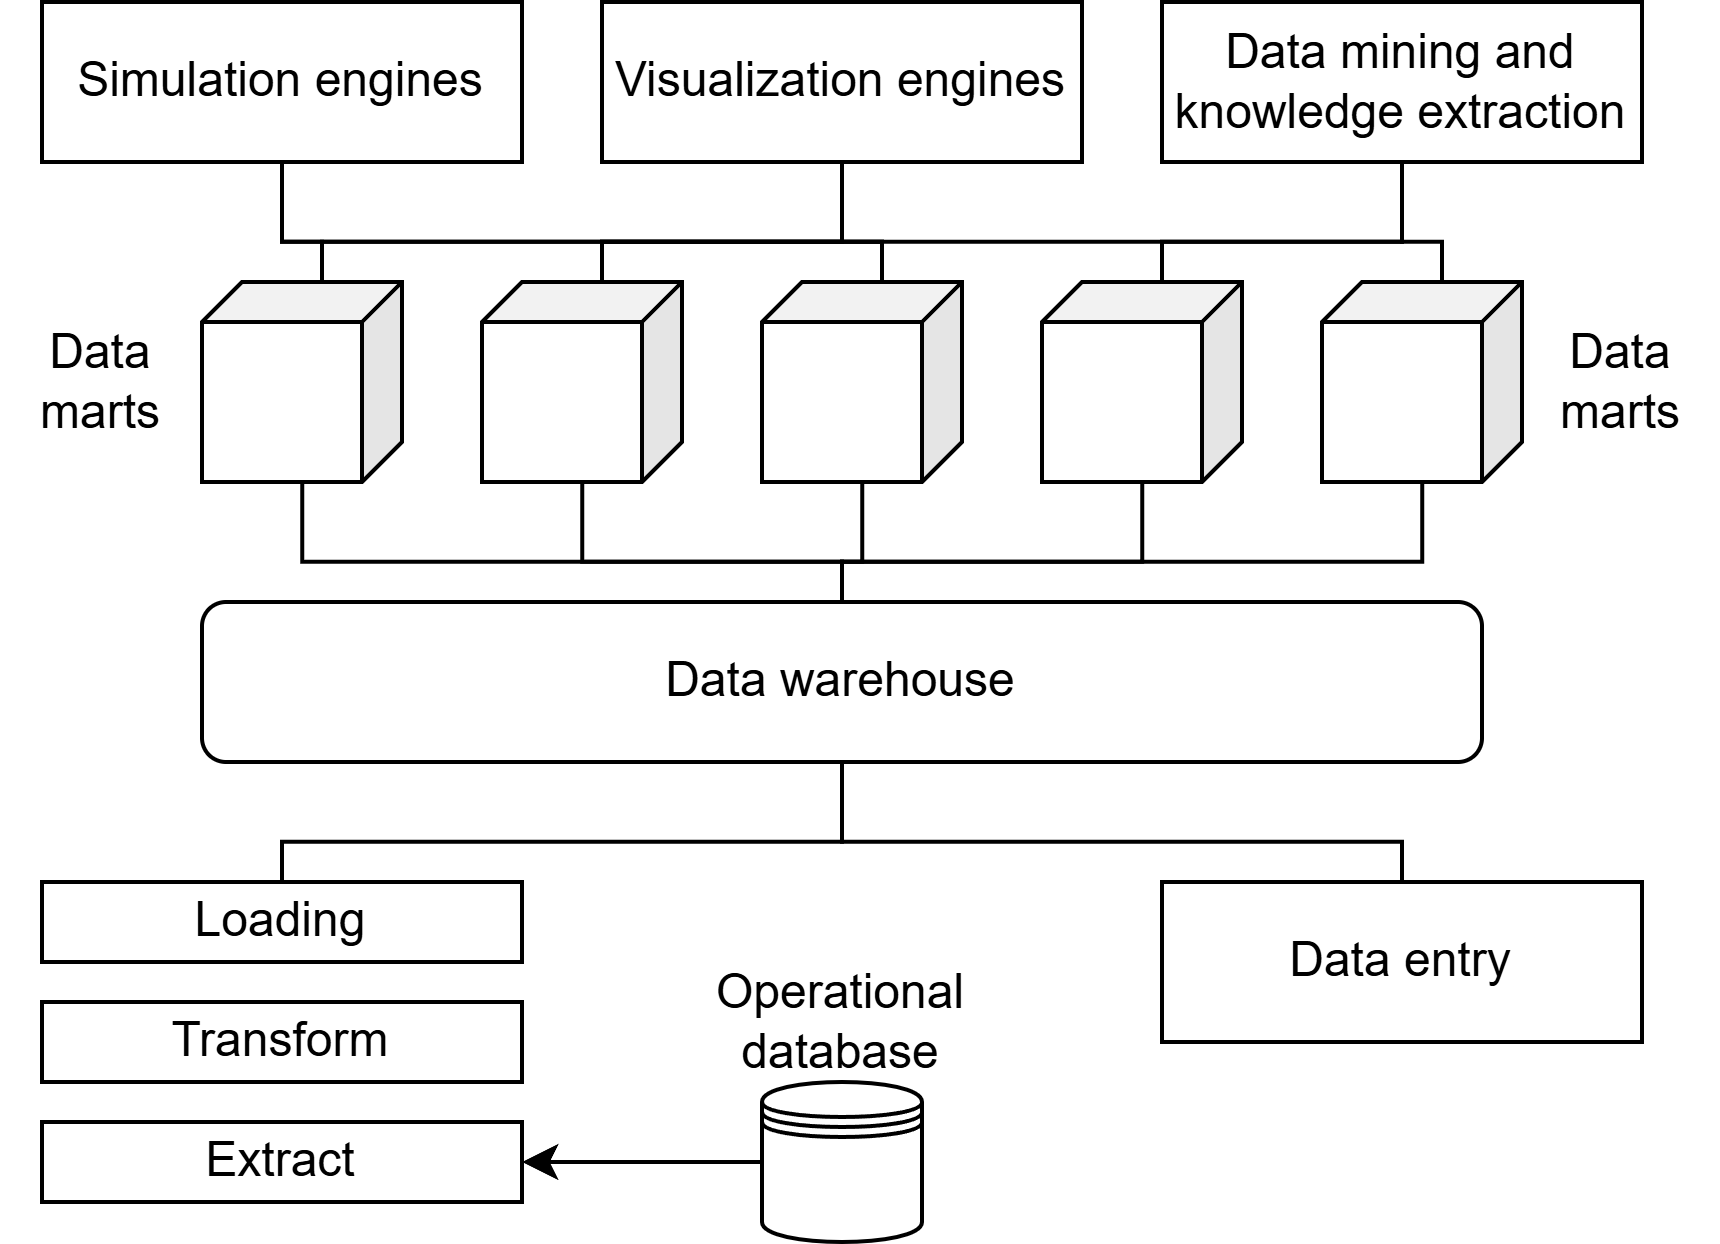
\includegraphics[width=0.5\linewidth]{images/bis4.png}
    \caption{Technological architecture}
\end{figure}
Information in data warehouses
June 2009
• Key Performance Indicators, i.e. aggregate information providing a summary
evaluation of a set of production activities or performance parameters
• Indicators have a value defined by different dimensions, including:
– Time (extension and granularity)
– Organizational unit
– Customer
– Product
– Process and activity
– Other dimensions such as channel, geographical area, project…

\subsection{Design}
Design steps of executive information systems
\begin{itemize}

\item Business requirements (key performance indicators)
\item Information sources: Operational DBs represent the main sources of
                    information. They include:
                    1. ERP operational data
                    2. CRM data
                    3. Operational information from custom
                    applications
                    4. Operational information from legacy applications
                    5. Information from the administrative portfolio

                    \item Information transformation: 1. Selection of source data
        2. Data quality control and data cleaning
        3. Data integration
        4. Data aggregation
\item Information storage: 1. Load is periodical, e.g. daily in our running example
2. Data are loaded in a data warehouse and subsequently copied in a smaller
database called data mart to improve time performance
3. Data warehouses and data marts may have different schemas and involve
an additional transformation step
1. Fact tables store the value of indicators
2. Keys represent the dimensions that can describe facts
3. The properties of keys are described in key tables
– Table of facts
– Table of keys
– Data warehouse design: Source selection 2 Target data design
Mapping tables from source
data to target data
Implementation of
transformation code 
Creation of Data Warehouse
6 Data extraction and load

\item Processing level
– Presentation and reporting
– Decision support engines
– Visualization engines
– Knowledge extraction engines
The processing level includes:
1. Engines
2. Mining and knowledge
extraction
3. Reporting

\end{itemize}
\subsubsection{CSF method}
CSF stands for critical success factor
• A critical success factor is a business decision variable critical
for the success of the whole company, i.e. a must for success
(necessary condition)
• The CSF method is a requirements analysis and specification
method for executive information systems
CSFs are an abstract concepts, such as:
– Security of cars
– Dependability of cars
– Design appeal of cars
• CSFs are complex constructs and correspond to multiple KPIs
1. Pre-definition: desk analysis
2. Interview: with top managers, aimed at identifying CSFs
3. Robustness analysis: aimed at selecting KPIs
4. Refinement and documentation: presentation to customer,
possible modifications, specification (written, but informal)
robustness analysis
Criteria to evaluate/select KPIs:
• Cost of information (e.g. customer satisfaction is costly)
• Significance, that is contribution to understand corresponding CSF
• Frequency, if information is seldom updated, KPI should be eliminated
• Structuredness, quantitative is preferred against qualitative